\documentclass[20pt,a1paper,landscape]{tikzposter}

% required packages
\usepackage{amsmath}
\usepackage{amsfonts}
\usepackage{amsthm}
\usepackage{graphicx}
\usepackage{natbib}
\usepackage{url}
\usepackage{booktabs}

% compact bibliography
\renewcommand{\bibsection}{}
\setlength{\bibsep}{0pt plus 0.3ex}

%% Available themes: see also
%% https://bitbucket.org/surmann/tikzposter/downloads/themes.pdf
\usetheme{Default}
\colorlet{backgroundcolor}{white}

% title information
\title{Guidance on Individualized Treatment Rule Estimation in High Dimensions}
\author{Philippe Boileau$^1$, Ning Leng$^2$, Sandrine Dudoit$^3$}
\institute{$^3$McGill University; $^2$Genentech Inc; $^3$University of California, Berkeley}

% dictate default block options
\newcommand{\myblock}[2]{\block[titleinnersep=2mm, linewidth=0.5mm]{#1}{#2}}
\newcommand{\mysmallblock}[2]{\block[titleinnersep=1mm, linewidth=1mm, bodyinnersep=5mm, roundedcorners=12, ]{{\small #1}}{{\tiny#2\par}}}

\begin{document}

\maketitle[width = 30in]
%% \node[anchor=west] at (TP@title.west) {
\includegraphics[width=6cm]{logos/mcgill_sig_red}};
%% \node[anchor=east] at (TP@title.east) {
\includegraphics[width=6cm]{logos/cal}};


\begin{columns}

  \column{0.333}

  \myblock{Motivation}{
    \begin{itemize}
      \itemsep2pt
        \item First Item
    \end{itemize}
  }

  \column{0.334}

  \myblock{Problem Formulation}{

    Other block

  }

  \myblock{Estimators}{
    \vspace{-1.5cm}
    \begin{tikzfigure}
      \centering
      \resizebox{0.28\textwidth}{!}{%
        \begin{tabular}{
            |p{0.1\textwidth} || p{0.3\textwidth}|
          }
          \hline
          CATE Estimator
          & Details \\
          \hline\hline
          Plug-In LASSO
          & A plug-in estimator using the LASSO. \\
          \hline
          Plug-In XGBoost
          & A plug-in estimator using XGBoost. \\
          \hline
          Modified Covariates LASSO
          & A modified covariates estimator using the LASSO. The propensity
          score is estimated using the logistic LASSO. \\
          \hline
          Modified Covariates XGBoost
          & A modified covariates estimator using XGBoost. The propensity
          score is estimated using the logistic LASSO. \\
          \hline
          Augmented Modified Covariates LASSO
          & An augmented modified covariates estimator using the LASSO. The propensity
          score is estimated using the logistic LASSO. \\
          \hline
          Augmented Modified Covariates XGBoost
          & An augmented modified covariates estimator using XGBoost. The propensity
          score is estimated using the logistic LASSO. \\
          \hline
          AIPW-based LASSO
          & An AIPW-based estimator using Super Learners to estimate the
          expected conditional outcome and the propensity score. Differences
          in predicted pseudo-outcomes are modelled using the LASSO. \\
          \hline
          AIPW-based Super Learner
          & An AIPW-based estimator using Super Learners to estimate the
          expected conditional outcome and the propensity score. Differences
          in predicted pseudo-outcomes are modelled using a Super Learner. \\
          \hline
          Causal Random Forests
          & A causal random forest estimator using cross-validation for
          hyperparameter selection. \\
          \hline
      \end{tabular}}
    \end{tikzfigure}
    \vspace{-1.0cm}
  }

  \myblock{Simulated Data-Generating Processes}{

    Setting $p=500$, we define 16 DGPs using every possible combination of the
    following factors:

    \begin{equation*}
      \resizebox{0.29\textwidth}{!}{$%
        \begin{split}
          \Sigma_{1} & = I_{500 \times 500} \\
          \Sigma_{2} & = \text{Block diagonal} \\
        \end{split}
        \quad \times \quad
        \begin{split}
          \pi_{1}(W) & = \frac{1}{2} \\
          \pi_{2}(W) & = \text{logit}^{-1}\left(\frac{W_{1} + W_{2} + W_{3} + W_{4}}{5}\right) \\
        \end{split}
        \quad\times\quad
        \begin{split}
          \mu_{1}(A, W) & = A + \gamma^{\top}W + (\delta^{(10)})^{\top}WA \\
          \mu_{2}(A, W) & = A + \gamma^{\top}W + (\delta^{(50)})^{\top}WA \\
          \mu_{3}(A, W) & = \gamma^{\top}W + 2\;\text{arctan}\left\{(\delta^{(10)})^{\top}WA\right\} \\
          \mu_{4}(A, W) & = \gamma^{\top}W + 2\;\text{arctan}\left\{(\delta^{(50)})^{\top}WA\right\} \\
        \end{split}$%
      }
    \end{equation*}

    where $\gamma_{1} = \ldots = \gamma_{5} = 2$, $\gamma_{6} = \ldots =
    \gamma_{500} = 0$, $\delta^{(10)}_{1} = \ldots = \delta^{(10)}_{10} = 2$,
    $\delta^{(10)}_{11} = \ldots = \delta^{(10)}_{500} = 0$, $\delta^{(50)}_{1}
    = \ldots = \delta^{(50)}_{50} = 1/2$, and $\delta^{(50)}_{51} = \ldots =
    \delta^{(50)}_{500} = 0$. $\Sigma_{2}$ is constructed by randomly generating
    $50$ positive definite square symmetric matrices with diagonal elements
    equal to one.

  }

  \column{0.333}

  \myblock{Results Snapshot}{
    \vspace{-1.5cm}
    \begin{tikzfigure}
      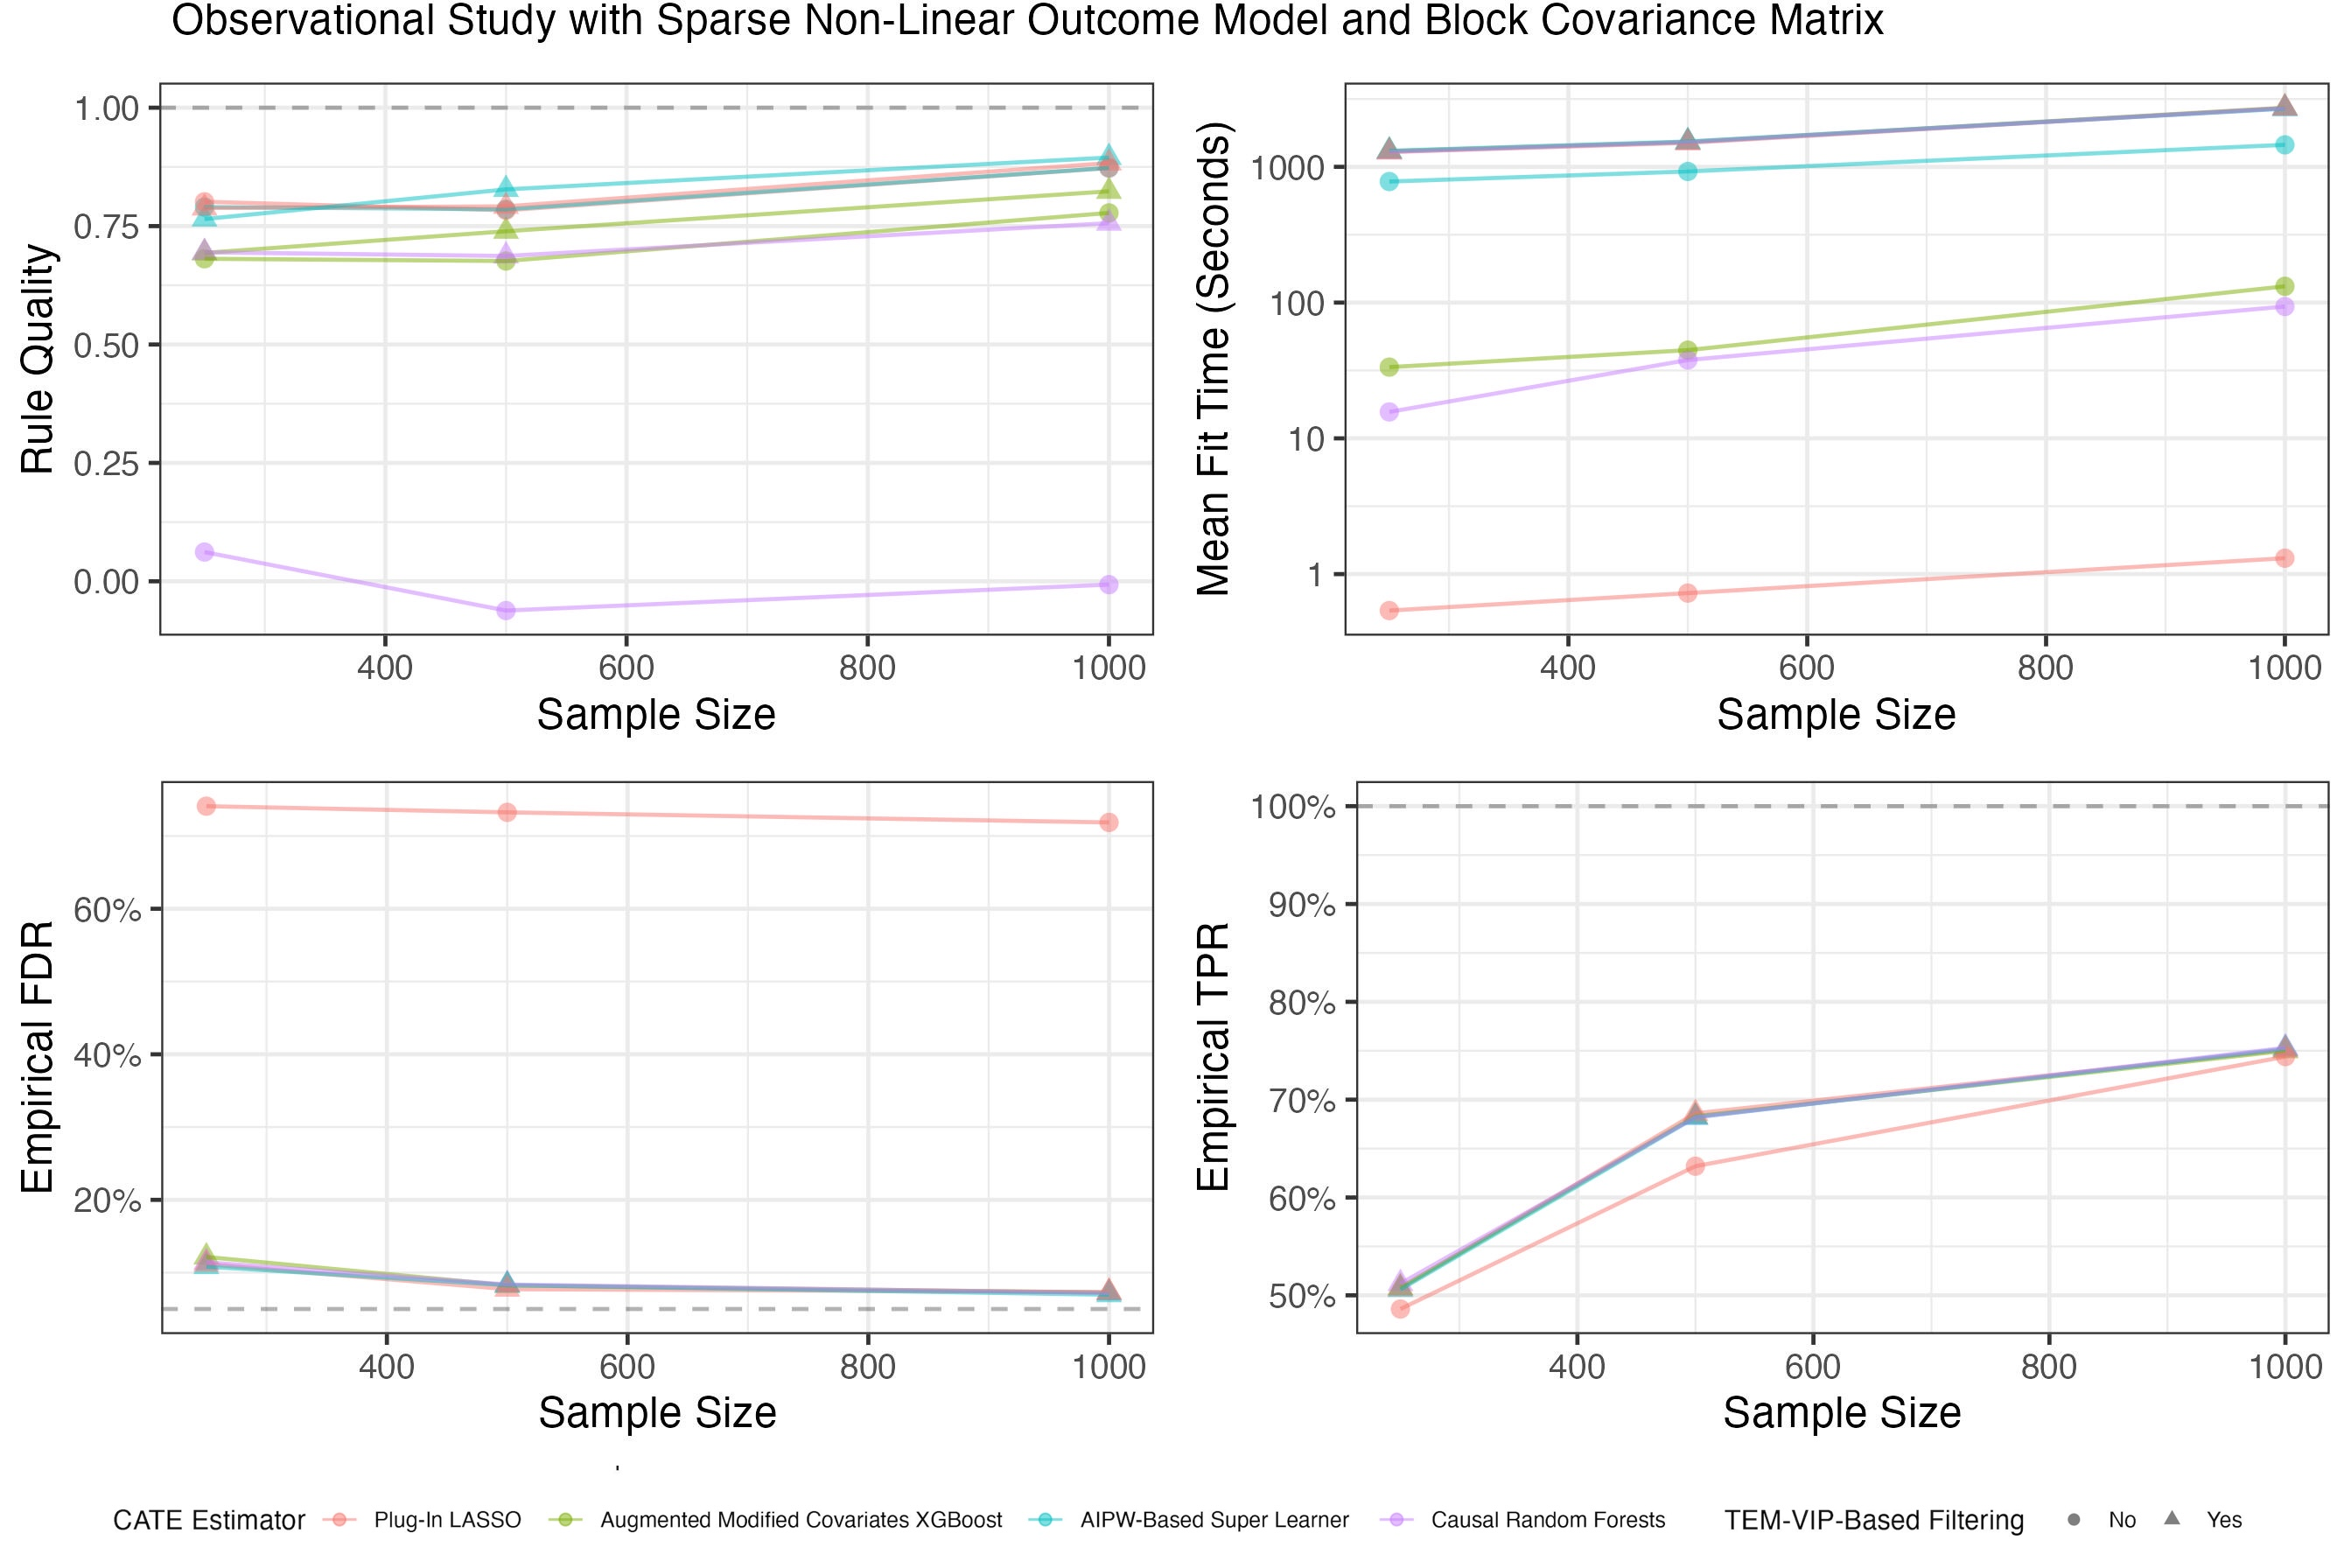
\includegraphics[width=0.29\textwidth]{figs/summary-plot.jpeg}
    \end{tikzfigure}
    \vspace{-1.0cm}
  }

  \myblock{Practical Guidance}{

    No estimator uniformly dominates others; tradeoffs must be made. Since rule
    quality is generally of primary concern, our results indicate that
    practitioners must choose between accurate interpretability and
    computationally efficiency. We provide the following guidance:

    \begin{itemize} \itemsep2pt

    \item \textbf{High-quality and accurately interpretable:} The filtered
      LASSO-based plug-in and AIPW-based estimators generally produce
      high-quality ITR estimates while accurately recovering TEMs. These
      estimators are computationally intensive, however.

    \item \textbf{High-quality and computationally efficient:} The LASSO-based
      plug-in estimator produces among the most high-quality rules in our
      simulation studies, providing empirical evidence that it is robust to
      model misspecification while being exceptionally computationally
      efficient. This estimator's built-in feature selection capabilities should
      not be used for TEM discovery, however.

    \end{itemize}
  }

  \mysmallblock{References}{
    \vspace{-3em}
    %% \bibliographystyle{unsrtnat}
    %% \bibliography{refs}
    \vspace{-1em}
  }

\end{columns}

\end{document}
